\documentclass[12pt]{article}
\usepackage{lingmacros}
\usepackage{tree-dvips}
\usepackage[utf8x]{inputenc} % Включаем поддержку UTF8 
\usepackage[russian]{babel} 
\usepackage{mathtools}
\usepackage{graphicx}
\usepackage{amsmath}

\graphicspath{{pict/}}
\DeclareGraphicsExtensions{.pdf,.png,.jpg}

\DeclarePairedDelimiter{\ceil}{\lceil}{\rceil}

\begin{document}

\section*{Решения}

\subsection*{Задача 1.1}
Если мы имеем n внешне одинаковых объектов, после одного взвешивания останется в худшем случае $\ceil{n}$ объектов, среди которых есть отличающийся по весу. Таким образом, если $n = 12$, то, в худшем случае, понадобятся 3 взвешивания $12\Rightarrow 4\Rightarrow 2\Rightarrow 1$.
Ответ: 3.

\subsection*{Задача 1.2}
Пусть номер квартиры равен $\overline{abc} = 100\cdot a + 10\cdot b + c$, где $a$, $b$ и $c$ -- цифры числа. Число с перевернутыми двумя последними цифрами при этом будет равно $\overline{acb} = 100\cdot a + 10\cdot c + b$. Затем решим уравнение в целых числах 
$$100 \cdot a + 10\cdot b + c + 100\cdot a + 10\cdot c + b = 1187,$$ 
$$200 \cdot a + 11\cdot b + 11\cdot c = 1187$$ с учетом ограничений на то, что $a$, $b$ и $c$ -- цифры в десятичной системе счисления.
$$200\cdot a + 11\cdot (b + c) = 200 \cdot 5 + 11 \cdot 17.$$
Таким образом, возможные номера квартир $589$ и $598$. Выбираем наименьший -- 589.
Ответ: 589.

\subsection*{Задача 1.3}
Пусть N -- количество учащихся в классе, А -- количество юношей в классе. Вероятность того, что оба дежурных окажутся мальчиками составляет 
$$P = \frac{A}{N}\cdot \frac{A - 1}{N - 1}.$$
Подставим из условия $N = 25$, $P = 3/25$ и получим следующее уравнение:
$$\frac{A}{25}\cdot\frac{A - 1}{24} = \frac{3}{25},$$
$$A^2 - A - 3 \cdot 24 = 0.$$
Уравнение имеет только один положительный корень $A = 9$. Значит, девочек в классе $25 - 9 = 16$. Ответ: 16.

\subsection*{Задача 1.4}
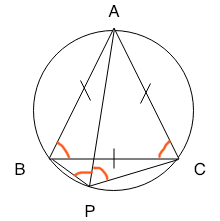
\includegraphics{math14_2}

Так как $\triangle ABC$ -- равносторонний, то $\angle BAC = \angle ABC = \angle ACB = 60^{\circ}$ и $AB = AC$. $\angle ABC = \angle APC$, так как опираются на $\smile AC$. $\angle ACB = \angle APB$, так как опираются на $\smile{AB}$. Таким образом, $\angle APB = \angle APC = 60^{\circ}$. По теореме косинусов 

\begin{equation*} 
    \begin{cases}
    AB^2 = AP^2 + BP^2 - 2 \cdot AP\cdot BP\cdot \cos(\angle APB),\\
    AC^2 = AP^2 + CP^2 - 2 \cdot AP\cdot CP\cdot \cos(\angle APC).
    \end{cases}
\end{equation*}

Так как $AB = AC$ и $\angle APC = \angle APB = 60^{\circ}$, получим:

$$AP^2 + BP^2 - AP\cdot BP\cdot = AP^2 + CP^2 - AP\cdot CP,$$
$$BP^2 - CP^2 = AP\cdot (BP - CP),$$
$$AP = BP - CP.$$
Подставим значения $BP = 3$ и $CP = 4$ и получим $AP = 7$. Ответ: 7.

\subsection*{Задача 1.5}
Пусть на доске записаны 4 числа $a$, $b$, $c$ и $d$. Пусть НОД$(a, b) = 2$, тогда НОД$(c, d) = 4$ быть не может, так как НОД всех пар будет кратным 2. Значит, пусть НОД$(a, c) = 4$ и тогда $d$ будет нечётным числом.
Исходя из записанных равенств, можно выписать следующие:
$$a = 4\cdot a_4 = 2 \cdot a_2$$
$$b = 2\cdot b_2$$
$$c = 4\cdot c_4$$
При этом НОД$(a_2, b_2) = 1$ и НОД$(a_4, c_4) = 1$. Очевидно также, что НОД$(b, c) = 2 \cdot x$ -- то есть это последняя искомая пара. Попробуем подобрать значения $a$, $b$, $c$ и $d$ так, чтобы они удовлетворяли всем равенствам и из НОД оставшихся пар равнялись указанным значениям. Например, $a = 4$, $b = 10$, $c = 12$ и $d = 15$. Таким образом, наименьшее возможное значение равно 2. Ответ: 2.

\subsection*{Задача 1.6}
Пусть загаданное число $X = A \cdot B$, где $A$ -- наименьший делитель, $B$ -- наибольший. Тогда $A + 77 = B$. $X = A \cdot (A + 77) \to min$. Так как $A \neg 1$, то минимум достигается при $A = 2$. Таким образом, $X = 2 \cdot 79 = 158$. Ответ: 158.  
\subsection*{Задача 1.7}
Каждая комбинация цифр на циферблате отображается ровно $1$ минуту, следовательно в задаче требуется найти количество соответствующих комбинаций. В группе цифр, отображающей часы может встретиться только $0$ или $1$ тройка. В остальных -- $0$, $1$ или $2$. Четыре тройки можно получить из следующих комбинаций: $X_1 = Q([0]:[2]:[2])$, $X_2 = Q([1]:[1]:[2])$, $X_3 = Q([1]:[2]:[1])$. $Q$ -- количество комбинаций в соответствии с количеством троек в группах цифр циферблата, соответствующих часам, минутам, секундам. $X_1 = 21 \cdot 1 \cdot 1$. $X_2 = 3 \cdot 14 \cdot 1$. $X_3 = 3 \cdot 1 \cdot 14$. $X = X_1 + X_2 + X_3 = 21 + 42 + 42 = 105$. Ответ: 105.

\subsection*{Задача 1.8}
$$x^3 + y^3 = 4(x^2y + xy^2 + 1),$$
$$(x+y)(x^2-xy+y^2) - 4xy(x + y) = 4,$$
$$(x+y)(x^2-5xy+y^2) = 4.$$
В левой части множители могут принимать только следующие пары значений: (-4, 1), (-2, -2), (-1, -4), (1, 4), (2, 2), (4, 1). Все 6 систем уравнений не дают целых корней. Ответ: 0. 

\subsection*{Задача 1.9}
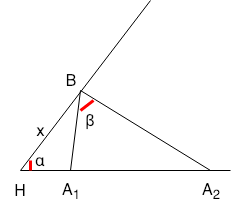
\includegraphics{math19}\\
Обозначим $\alpha = \angle BAA_2=60^{\circ}$, $\beta = \angle A_1BA_2$, $x = BH$. По теореме косинусов выразим $A_1B$ и $A_2B$ и подставим значения $A_1 = 2B$ и $A_1A_2 = 8$ из условия:
$$A_1B^2 = x^2 + A_1H^2 - 2xA_1H\cdot \cos\alpha = x^2 + 4 - 2x,$$
$$A_2B^2 = x^2 + A_2H^2 - 2xA_2H\cdot \cos\alpha = x^2 + 100 - 10x.$$
Рассмотрим $\triangle A_1BA_2$, по теореме косинусов:
$${A_1A_2}^2 = A_1B^2 + A_2B^2 - 2A_1B\cdot A_2B \cos\beta.$$
Выразим $\cos\beta$:
$$\cos\beta = \frac{A_1B^2 + A_2B^2 - {A_1A_2}^2}{2A_1B\cdot A_2B} = \frac{x^2 + 4 - 2x + x^2 + 100 - 10x - 64}{2\sqrt{x^2 + 4 - 2x} \cdot \sqrt{x^2 + 100 - 10x}} =  $$
$$=\frac{x^2 - 6x + 20}{\sqrt{x^2 + 4 - 2x} \cdot \sqrt{x^2 + 100 - 10x}}.$$
Для максимизации острого угла $A_1BA_2$ требуется, найти $x$, при котором достигается $min(\cos\beta)$. Решим уравнение $(\cos\beta)'_x = 0$ и найдем точку минимума. $x = 2\sqrt{5} \approx 4.472135955$. Ответ: 4.472135955.
\subsection*{Задача 1.10}
Расстояние между точкой с координатами $(x_0, y_0, z_0)$ и плоскостью, задаваемой уравнением $Ax + By + Cx + D = 0$ вычисляется по формуле:
$$S = \frac{|Ax_0+By_0+Cz_0 + D|}{\sqrt{A^2+B^2+C^2}}$$
Для заданных точки и плоскости $$S = \frac{|2 \cdot 0 + 4 \cdot 3 - 4 \cdot 6 - 6|}{\sqrt{2^2 + 4^2 + 4^2}} = 3.$$ Ответ: 3.
\end{document}